\documentclass[man, floatsintext]{apa7}
\usepackage[american]{babel}
\usepackage{csquotes}
\usepackage{amsmath,amsthm,bm,bbm}
\usepackage[justification=centering]{subcaption}
\usepackage[justification=centering]{caption}
\usepackage[style=apa, backend=biber]{biblatex}
\addbibresource{lit.bib}

\title{Conditionally Unbiased Best Linear Predictors for Score Augmentation}
\shorttitle{Score augmentation using CUBLP}
\authorsnames{Xiang Liu, Matthew S. Johnson, Sandip Sinharay}
\authorsaffiliations{Educational Testing Service}

%% new commands %%
\newcommand{\mbf}[1]{\bm{#1}}
\newcommand{\bc}{\mbf{c}}
\newcommand{\bX}{\mbf{X}}
\newcommand{\bY}{\mbf{Y}}
\newcommand{\bT}{\mbf{T}}
\newcommand{\C}{\mathcal{C}}
\newcommand{\bbeta}{\mbf{\beta}}
\newcommand{\bmu}{\mbf{\mu}}
\newcommand{\beps}{\mbf{\epsilon}}
\newcommand{\btau}{\mbf{\tau}}
\newcommand{\bgamma}{\mbf{\gamma}}
\newcommand{\blambda}{\mbf{\lambda}}
\newcommand{\bW}{\mbf{W}}
\newcommand\independent{\protect\mathpalette{\protect\independenT}{\perp}}
\def\independenT#1#2{\mathrel{\rlap{$#1#2$}\mkern2mu{#1#2}}}
\DeclareMathOperator{\MSE}{MSE}
\DeclareMathOperator{\Cov}{Cov}
\DeclareMathOperator{\Var}{Var}
%%%%%%%%%%% 

\abstract{The best linear predictor (BLP) has been proposed to combine
different types of information in estimating true scores. The BLP is
biased for individual examinees when conditioned on the true score. In this
paper, we propose a conditionally unbiased BLP. Additionally, a least square
method is introduced for parameter estimation.}

\begin{document}
  \maketitle

  \section{Introduction}
	With the current popular trend of transition from traditional paper-pencil
  assessments to digital formats, an increasingly common task is to combine
  different sources of information in assessing some latent construct. For
  instance, in the context of writing assessments, in addition to the final
  product essays, digital platforms are now able to capture information on
  keystrokes during
  students' interaction with writing tasks. Thus, features related to writing
  process are now becoming available (e.g. \cite{Zhang2019,Guo2019}).
  Furthermore, additional product features such as those related to natural
  language processing (NLP) could also be obtained through NLP programs (e.g.
  the e-rater\textsuperscript{\textregistered} program; 
  \cite{Attali2006,Burstein2004}). Then a natural question is whether and how
  different sources of information can be combined to augment the rater
  scores in making inferences on examinees' writing proficiency.

  There has been some previous research exploring related methods. For example,
  \textcite{Zhang2015} used linear regression to predict adjudicated essay
  scores from a large number of keystroke logging features and other product
  features. \textcite{Sinharay2019} examined the same prediction problem
  utilizing machine learning methods such as the random forests and boosting. A
  common assumption of these methods is that essay score, the prediction
  target, is treated as fixed and known. However, in educational and
  psychological measurement, prediction targets are almost always latent and
  measured with error. To address this issue, the best linear predictors (BLP;
  e.g. \cite{Haberman2015,Yao2019}) has been proposed to combine sources of
  information (e.g. scores from other sections) along with manifest variables
  such as the rater scoresand to predict some latent true score (e.g. the
  writing proficiency) .

  The BLP minimizes the mean squared error (MSE) of prediction among all linear
  predictors. An important property of the BLP is that, when averaged over the
  population, the expected prediction is equal to the expected true score. In
  other words, the BLP is unbiased. However, it exhibits shrinkage towards
  the population mean. Consequently, the BLP is biased conditional on the true
  score level. This may lead to some serious fairness concern as the BLP could
  favor certain groups of examinees over others.

  In this paper, we introduce a conditionally unbiased best linear predictor 
  (CUBLP) that minimizes the prediction error among all
  linear predictors that are unbiased at all true score levels. The proposed
  method is flexible and can be applied to a wide variety of problems.

  \section{Methods}
  Let $\bW = (\bY^\top, \bX^\top)^\top$ denote observed random variables
  from a random examinee where $\bY = (Y_1, Y_2, \dots, Y_J)^\top$ is the vector
  of variables measured with error\footnote{Commonly referred to as manifest
  variables of some latent trait, e.g. essay scores from raters.}
  and $\bX = (X_1, X_2, \dots, X_K)^\top$ is the vector of variables measured
  without error\footnote{Covariates that may correlate with the latent
  trait of interest, e.g. typing speed.}. For simplicity, we consider an
  unidimensional true score $S$ and further assume that $\bW$ and $S$ are
  linearly related, i.e.
  \begin{equation}
    \mbf{W} = \left (
      \begin{array}{c} \bY \\  \bX \end{array} \right ) =
    \mbf{\alpha} + \mbf{\lambda} S + \mbf{\epsilon}_w.
  \end{equation}
  We propose a CUBLP of $S$ in the form of $\gamma_0 + \mbf{\gamma}_1^\top 
  \mbf{W}$
  that minimizes
  \begin{equation}
  \label{eq:mse}
    \MSE = E\left [ ( S - \gamma_0 -\mbf{\gamma}_1^\top \mbf{W} )^2 \right],
  \end{equation}
  subject to the constraint that it is conditionally unbiased, that is
  \begin{equation}
  \label{eq:constraint}
    E[ \gamma_0 + \mbf{\gamma}_1^\top \mbf{W} | S ] = \gamma_0 + 
    \mbf{\gamma}_1^\top E[\mbf{W} | S ] = S.
  \end{equation}

  Under the assumption $E[\mbf{\epsilon}_w|S] = 0$, we have $E[\bW|S] =
  \blambda S$. Combined
  with the observation that, in order to minimize the MSE in Equation~
  \ref{eq:mse},
  $\gamma_0 = E[S] -
  \mbf{\gamma}_1^\top E[\mbf{W}]$, it leads to
  \begin{equation}
  \begin{gathered}
    S = E[S] - \mbf{\gamma}_1^\top \mbf{\lambda} E[S] + \mbf{\gamma}_1^\top
           \mbf{\lambda} \\
    S-E[S] = \mbf{\gamma}_1^\top \mbf{\lambda} (S - E[S]).
  \end{gathered}    
  \end{equation}
  It immediately follows that the constraint in Equation~\ref{eq:constraint}
  reduces to
  \begin{equation}
    \mbf{\gamma}_1^\top \blambda = 1.
  \end{equation}
  We solve the constrained minimization problem with the method of Lagrange
  multipliers (See Appendix~\ref{app:optim} for details). The CUBLP
  coefficients are
  \begin{equation}
  \label{eq:coef_cublp}
    \bgamma_{1} = \frac{\mbf{\Sigma}^{-1}_{\beps_w} \blambda}{
      \blambda^\top \mbf{\Sigma}^{-1}_{\beps_w} \blambda},
  \end{equation}
  where $\mbf{\Sigma}_{\beps_w}$ is the variance-covariance matrix of $\beps_w$.

  Notice that the CUBLP coefficients in Equation~\ref{eq:coef_cublp} are
  expressed as a function of the population parameters $\blambda$ and $
  \mbf{\Sigma}_{\beps_w}$. In almost all real applications, they have to be
  estimated. Let 
  \[ \blambda = \left (\begin{array}{r} \blambda_{\bY} \\
  \blambda_{\bX} \end{array} \right), \]
  where $\blambda_{\bY} = (\lambda_{Y_1},\lambda_{Y_2}, \dots, \lambda_
  {Y_K})^\top$ and $\blambda_{\bX} = (\lambda_{X_1}, \lambda_{X_2}, \dots,
  \lambda_{X_J})^\top$ are the loadings for $\bY$ and $\bX$.
  In many cases, it may be desirable or necessary to assume that $\lambda_{Y_j}
  = \lambda_Y, \forall j$. This equal discrimination assumption is common for
  many measurement models. For the equal discrimination cases, assuming $\bW$
  are standardized and under some additional assumptions, the least square (LS)
  estimator for $\blambda$ is
  \begin{equation}
    \hat{\lambda_Y} = \sqrt{\frac{\sum_{k \neq k'} r_{Y_k Y_{k'}}}{K(K-1)}}
  \end{equation}
  and
  \begin{equation}
    \hat{\lambda_{X_j}} = \frac{\sum_k r_{Y_k X_j}}{K\hat{\lambda_Y}},
  \end{equation}
  where $r_{Y_k X_j}$ denotes the correlation between $Y_k$ and $X_j$. For
  unequal discrimination cases, the LS estimator can be obtained by iterating
  through
  \begin{equation}
    \hat{\lambda_{Y_k}} = \frac{\sum_{k' \neq k} \lambda_{Y_{k'}} r_{Y_{k}Y_{k'}} +
    \sum_j \lambda_{X_j} r_{Y_k, X_j}}{\sum_{k' \neq k} \lambda_{Y_{k'}}^2 + \sum_j
    \lambda_{X_j}^2},
  \end{equation}
  and
  \begin{equation}
    \hat{\lambda_{X_j}} = \frac{\sum_k \lambda_{Y_k} r_{Y_k X_j}}{\sum_k \lambda_
    {Y_k}^2}
  \end{equation}
  until convergence. A natural choice of an estimator for the residual
  covariance matrix is then 
  \begin{equation}
    \hat{\mbf{\Sigma}_{\beps_w}} = \mbf{\Sigma}_{\bW} - \hat{\blambda} 
    \hat{\blambda}^\top.
  \end{equation}
  For a sketch of the derivations of these results, please see Appendix~
  \ref{app:estimation}.

  \section{Planned simulations and data analysis}
  We plan to conduct simulation studies to examine the properties of the
  proposed CUBLP and the LS estimator of the parameters. preliminary results 
  suggest that the proposed LS estimator has good statistical properties (See
  Figure~\ref{fig:ls_bias_var}). 
  \begin{figure}
    \centering
    \begin{subfigure}[b]{0.4\textwidth}
      \centering
      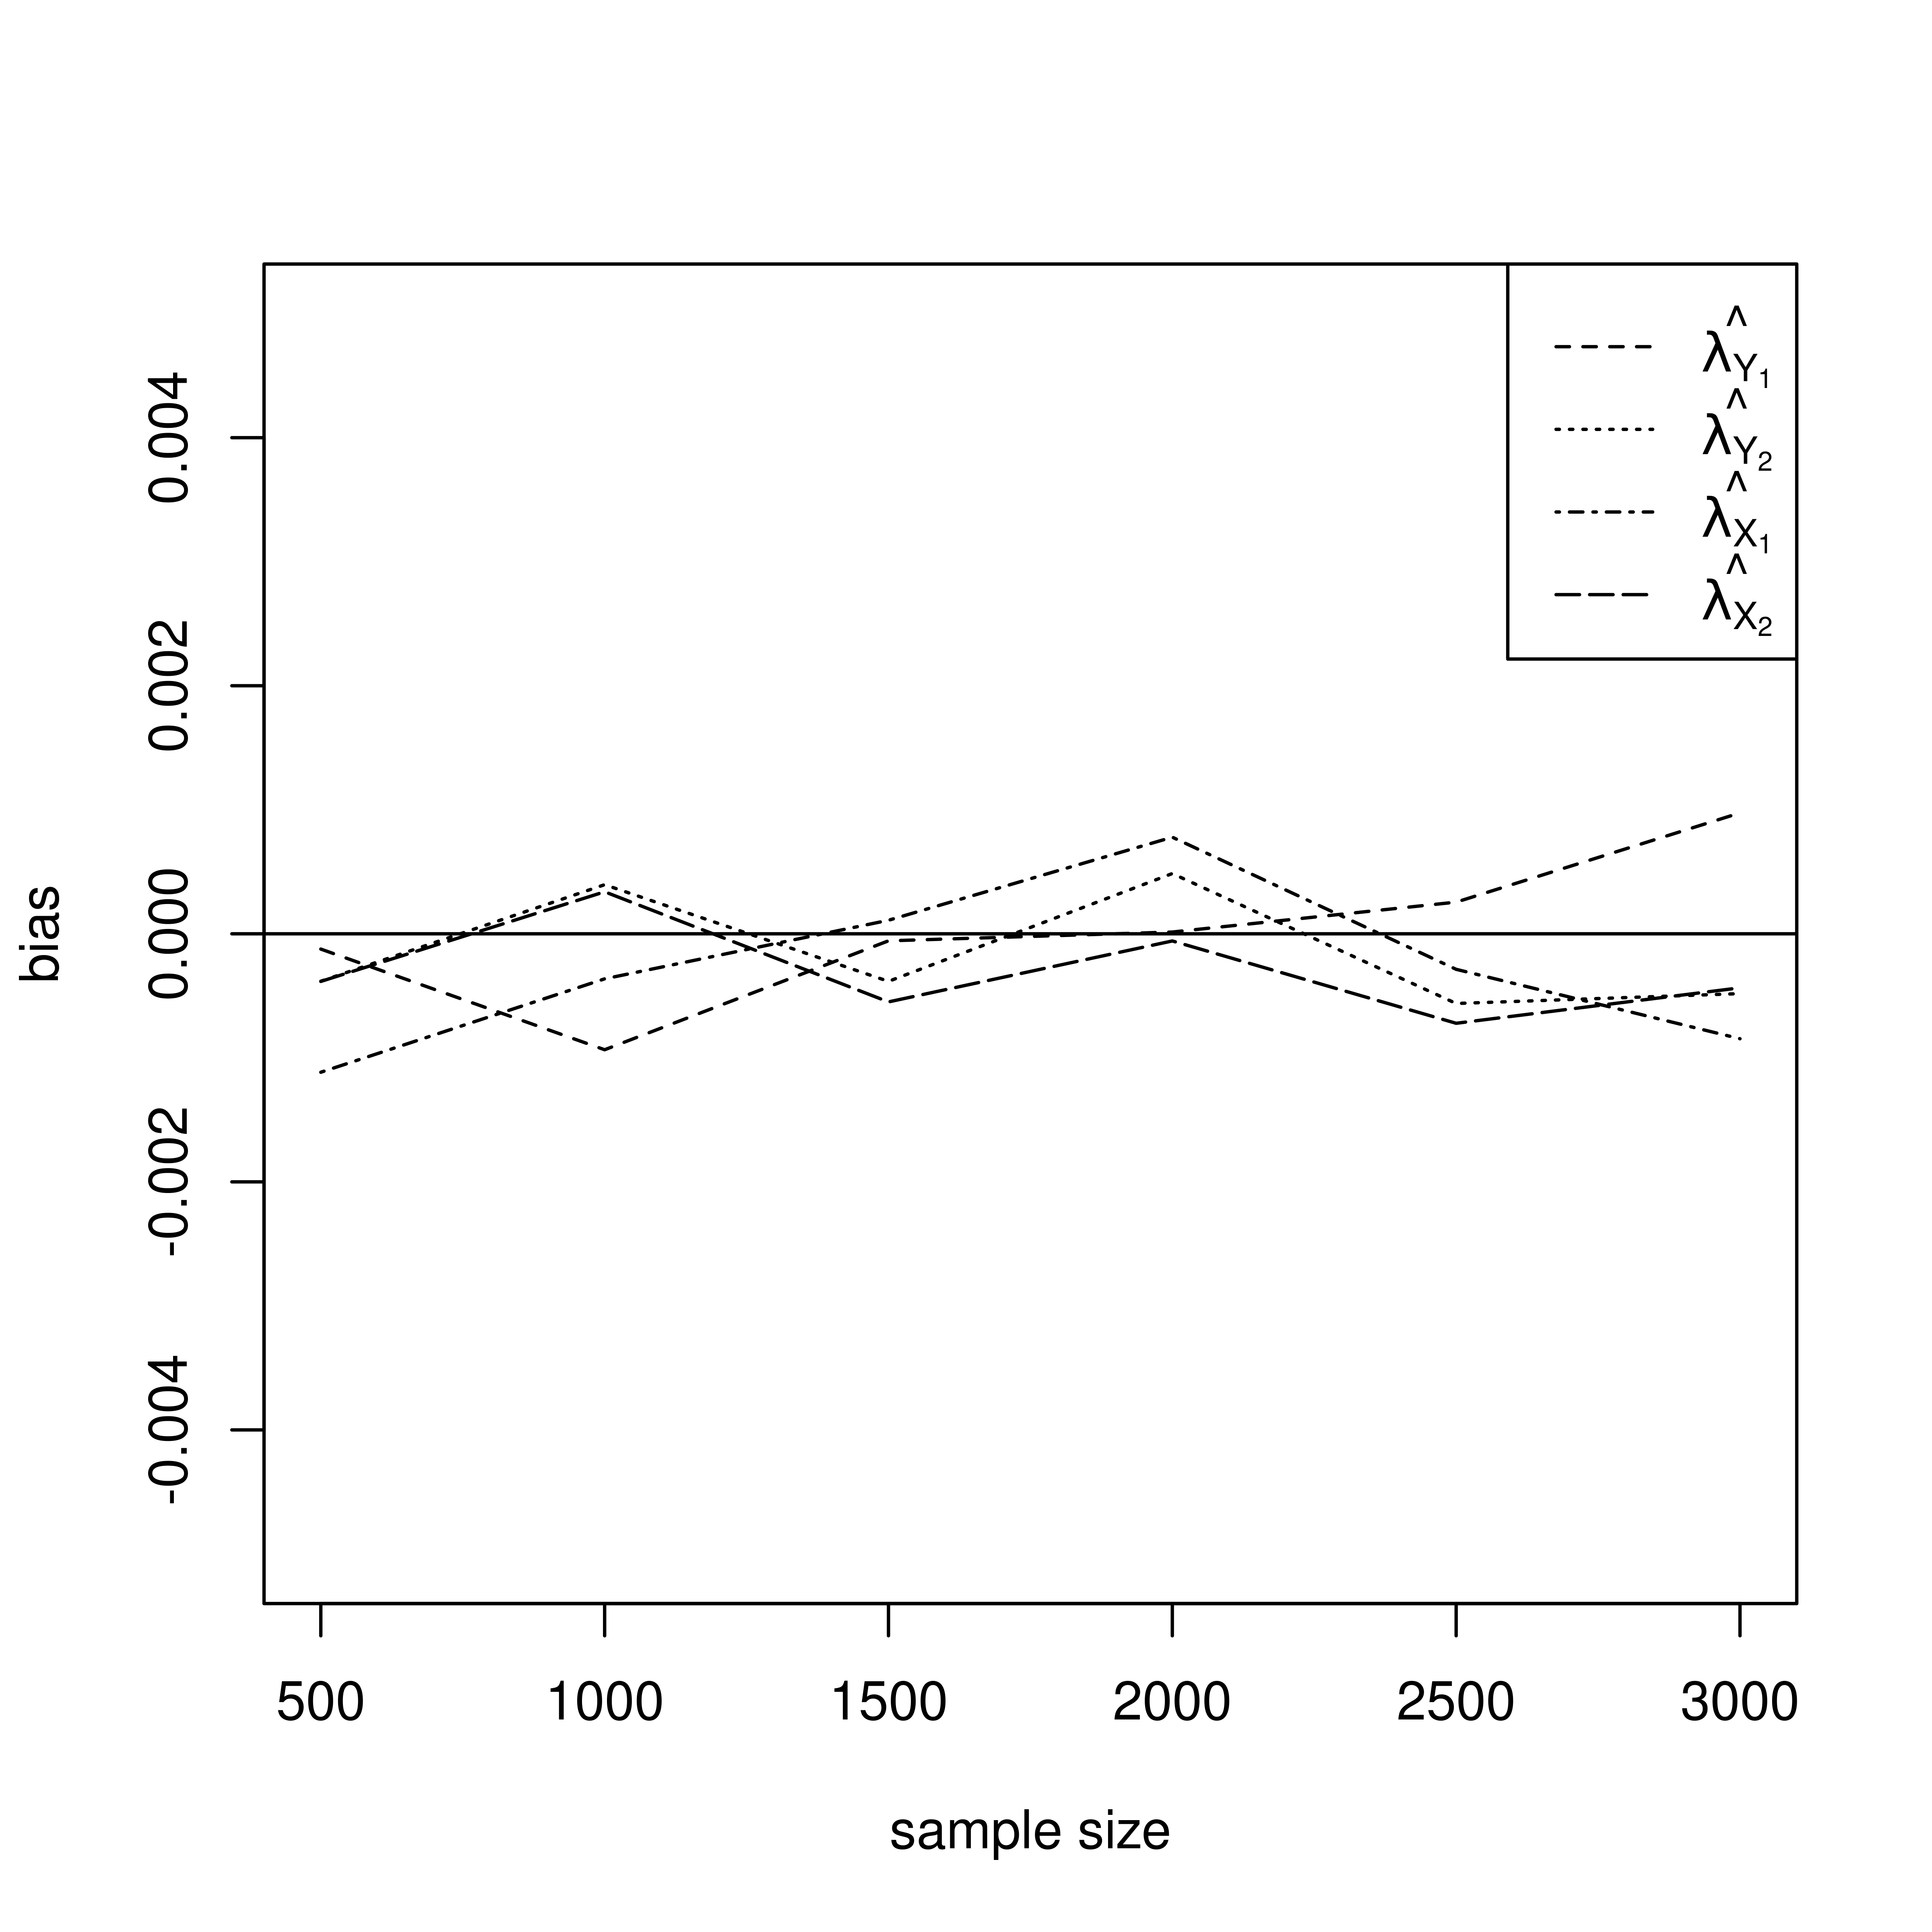
\includegraphics[width=\textwidth]{bias_uneq_discrim_high.png}
      \caption{Bias}
    \end{subfigure}
    \begin{subfigure}[b]{0.4\textwidth}
      \centering
      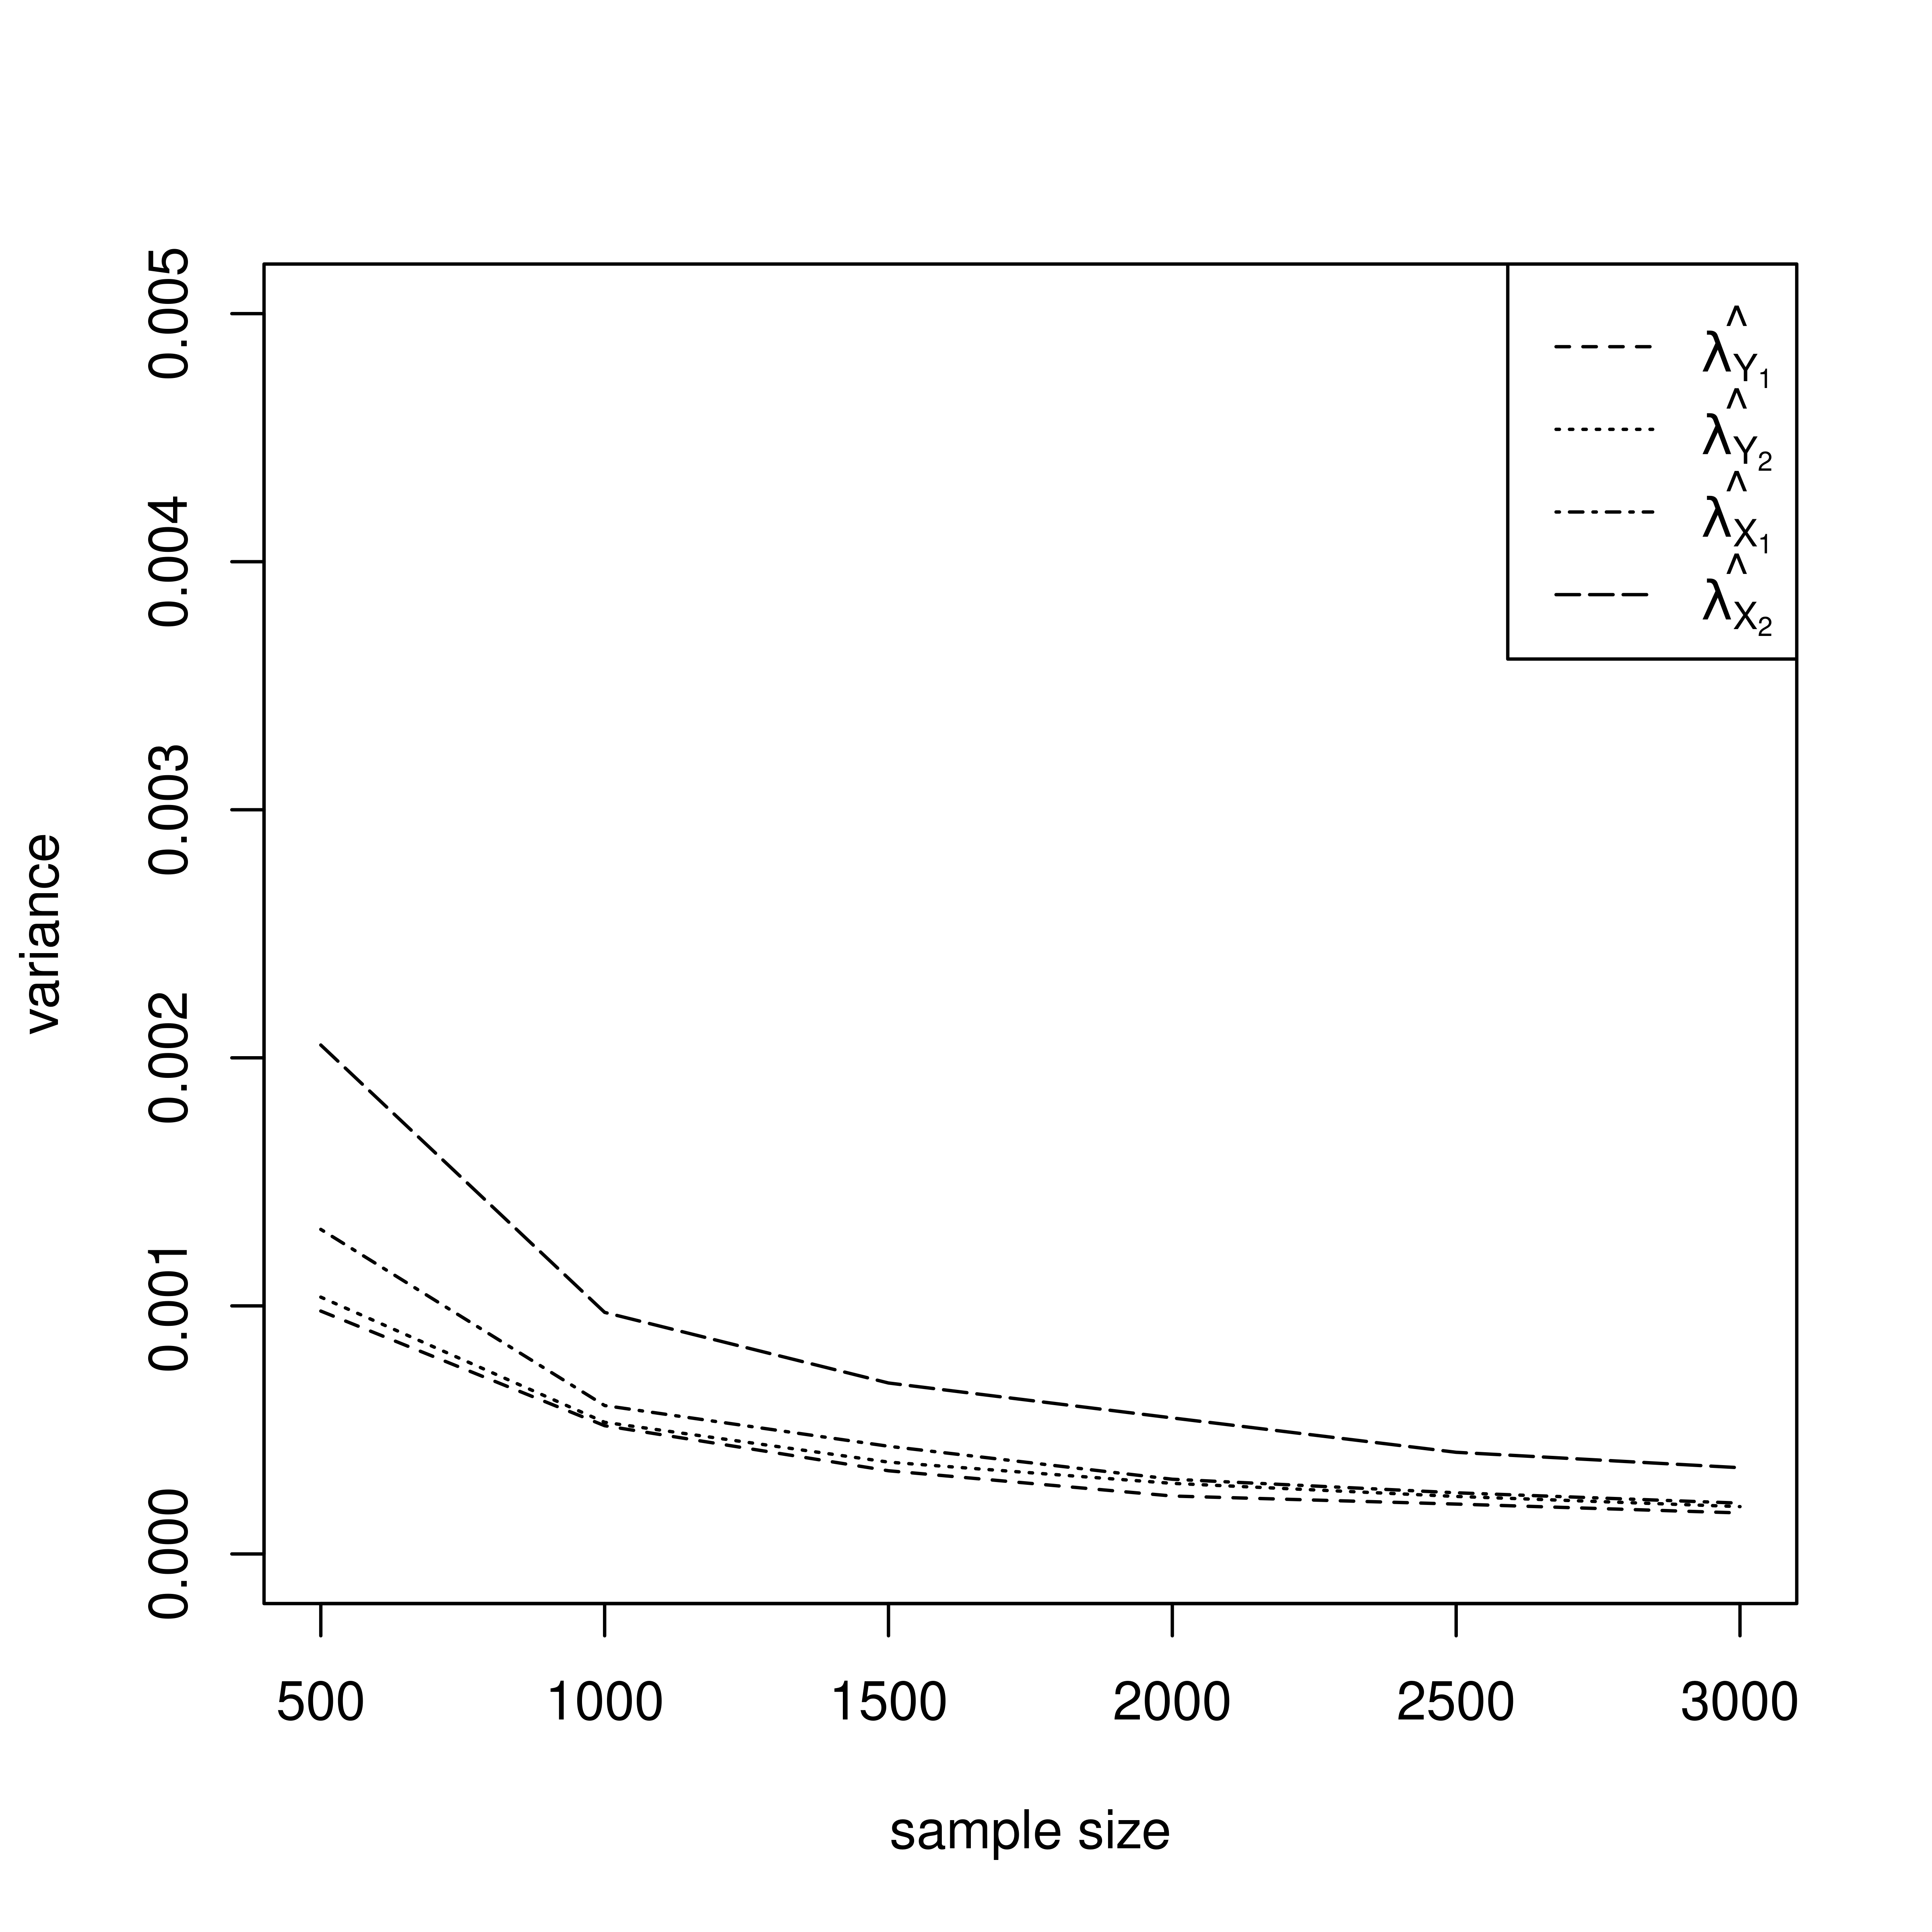
\includegraphics[width=\textwidth]{var_uneq_discrim_high.png}
      \caption{Variance}
    \end{subfigure}
    \caption{Bias and variance of the LS estimator}
    \label{fig:ls_bias_var}
  \end{figure}
  Further simulation studies would investigate the prediction performance of the
  CUBLP under different scenarios, e.g. different sample sizes, high/low
  correlations between the manifest variables $\bY$ and the true score $S$.
  Prediction bias and variance would be examined. We will also apply the
  proposed method to a real dataset from a pilot study of an
  English language test where examinees were asked to respond to several speech
  tasks. Each response was scored by two human raters. And NLP features would be
  used to augment the human rater scores in predicting the speaking proficiency.

  \section{Practical Implications}
  The proposed CULBP method utilizes multiple sources of information
  about the examinees to improve measurement precision. At the same time, it
  does it in an equitable fashion. This is particularly important when we
  develop methods that can leverage the opportunities that the current trend of
  Big Data brings.


  \printbibliography 
  \appendix
  \section{Constrained Minimization of the MSE}
  \label{app:optim}
  To find the optimal value for $\gamma$ we use a Lagrange multiplier
  approach where we optimize
  \[ \frac{1}{2} MSE - \delta (\mbf{\gamma}_1^\top \mbf{\lambda}-1 ) \]
  The gradient of this function is
  \[ - E\left [ (\mbf{W} - E[\mbf{W}] ) ( S -E[S] - 
      (\mbf{W} - E[\mbf{W}] )^\top \mbf{\gamma}_1) \right] - \delta
    \mbf{\lambda} \]
  Because $\mbf{W} = \mbf{\lambda} S + \beps_w $ and $\mbf{\lambda}^\top
  \mbf{\gamma} = 1$ by constraint, this gradient becomes
  \[ E \left [ (\bW - E[\bW]) \beps_w^\top \bgamma_1 \right ] - \delta
    \blambda \]
  \[ E \left [ (\blambda (S-E[S]) + \beps_w ) \beps_w^\top \bgamma_1 \right ] -
  \delta
    \blambda \]
  Therefore, the solution satisfies
  \begin{eqnarray*}
    \mbf{\Sigma}_{\beps_w} \bgamma_1 &=& \delta \blambda \\
    \bgamma_1 &=& \delta \mbf{\Sigma}^{-1}_{\beps_w} \blambda
  \end{eqnarray*}
  where $\delta$ is a constant to ensure the constraint is met.
  Therefore the CUBLP coefficients are
  \begin{equation}
    \bgamma_{1} = \frac{\mbf{\Sigma}^{-1}_{\beps_w} \blambda}{
      \blambda^\top \mbf{\Sigma}^{-1}_{\beps_w} \blambda}
    \label{eq:blup}
  \end{equation}
  where $\mbf{\Sigma}_{\beps_w} = \Cov(\beps_w)$ is the covariance of
  the error terms $\beps_w = \bW - \blambda S $.
  
  \section{Parameter estimation}
  \label{app:estimation}
  Following the results in the previous section, the BLUP estimator is a function of the factor loadings $\blambda$. However, this loading vector is generally unknown and has to be estimated. Here we consider the single score case.
  Let \[ \blambda = \left (\begin{array}{r} \blambda_{\bY} \\ \blambda_{\bX} \end{array} \right) \],
  where $\blambda_{\bY} = (\lambda_{Y_1}, \lambda_{Y_2}, \dots, \lambda_{Y_K})'$
  and $\blambda_{\bX} = (\lambda_{X_1}, \lambda_{X_2}, \dots, \lambda_{X_J})'$.
  Assume all observed variables are standardized and $E(S) = \mu_S = 0$ and
  $\sigma^2_{S} = 1$. It leads to
  \begin{equation} 
  \mbf{\Sigma}_{\bW} = \blambda \blambda' + \mbf{\Sigma}_{\beps}.
  \end{equation}
  We further assume that the covariance of $\bY$ is fully explained by $S$. That is
  \begin{equation}
    \mbf{\Sigma}_{\bY} = \blambda_{\bY} \blambda_{\bY}' + \mbf{\Psi}_{\bY},
  \end{equation}
  where $\mbf{\Psi}_{\bY}$ is a diagonal matrix with residual variances of $\bY$
  on the main diagonal. This is a common assumption for many popular measurement
  models. Now, we impose some additional restrictions on the residual covariance
  matrix $\mbf{\Sigma}_{\beps}$. $\bY$ is assumed to be uncorrelated with $\bX$
  given S. Equivalently, $\Cov(\beps_{\bY}, \beps_{\bX}) = \mbf{0}$.

  In many cases, it may be desirable or necessary to assume that $\lambda_{Y_j} = \lambda_{Y}$, $\forall j$. This equal discrimination assumption also simplifies the estimation of $\blambda$. Consider a quadratic loss function,
  \begin{equation}
    L(\blambda) = \sum_{k \neq k'} (\lambda_{Y}^2 - r_{Y_k Y_{k'}})^2 + \sum_k \sum_j (\lambda_Y \lambda_{X_j} - r_{Y_k X_j})^2.
  \end{equation}
  Taking the gradient to minimize the loss function,
  \begin{equation}
  \label{eq:loading_gradient_eqs}
    \nabla L = \left(
    \begin{array}{c} 4\lambda_Y \sum_{k \neq k'}(\lambda_{Y}^{2} - r_{Y_k Y_{k'}}) + 2K\lambda_Y\sum_j\lambda_{X_j}^2 - 2\sum_j \lambda_{X_j} \sum_k r_{Y_k X_j}\\
    \vdots\\
    2K\lambda_Y^2\lambda_{X_j} - 2\lambda_Y\sum_k r_{Y_k X_j}\\
    \vdots
    \end{array}\right) = \mbf{0}.
  \end{equation}
  Solving Equation \ref{eq:loading_gradient_eqs} leads to the unweighted least square estimator of the loadings,
  \begin{equation}
    \hat{\lambda_Y} = \sqrt{\frac{\sum_{k \neq k'} r_{Y_k Y_{k'}}}{K(K-1)}}
  \end{equation}
  and
  \begin{equation}
    \hat{\lambda_{X_j}} = \frac{\sum_k r_{Y_k X_j}}{K\hat{\lambda_Y}}.
  \end{equation}

  The solutions under unequal discriminations are
  \begin{equation}
    \hat{\lambda_{Y_k}} = \frac{\sum_{k' \neq k} \lambda_{Y_{k'}} r_{Y_{k}Y_{k'}} +
    \sum_j \lambda_{X_j} r_{Y_k, X_j}}{\sum_{k' \neq k} \lambda_{Y_{k'}}^2 + \sum_j
    \lambda_{X_j}^2},
  \end{equation} 
  and
  \begin{equation}
    \hat{\lambda_{X_j}} = \frac{\sum_k \lambda_{Y_k} r_{Y_k X_j}}{\sum_k \lambda_
    {Y_k}^2}
  \end{equation}

  
  \end{document}